% Created 2019-09-26 Thu 01:24
% Intended LaTeX compiler: pdflatex
\documentclass[10pt,t]{beamer}
\usepackage[utf8]{inputenc}
\usepackage[T1]{fontenc}
\usepackage{graphicx}
\usepackage{grffile}
\usepackage{longtable}
\usepackage{wrapfig}
\usepackage{rotating}
\usepackage{amsmath}
\usepackage{textcomp}
\usepackage{amssymb}
\usepackage{capt-of}
\usepackage{hyperref}
\usetheme{default}
\author{L. Larrabee Strow}
\date{\today}
\title{\large Insert into Andy's Talk}
\subtitle{\footnotesize{AIRS Science Team Meeting}}
\date{\vspace{0.1in}\footnotesize{September 26, 2019\vfill}}
\author{L. Larrabee Strow\inst{1,2} and Sergio De Souza-Machado, UMBC\inst{1,2}}
\institute[UMBC]{\inst{1} UMBC Physics Dept. \and \inst{2}UMBC JCET}
\input beamer_setup
\usetheme{metropolis}
\metroset{titleformat title=allcaps}
\renewcommand{\UrlFont}{\small\tt}
\renewcommand*{\UrlFont}{\footnotesize}
\tolerance=1000
\RequirePackage{fancyvrb}
\DefineVerbatimEnvironment{verbatim}{Verbatim}{fontsize=\footnotesize}
\hypersetup{
 pdfauthor={L. Larrabee Strow},
 pdftitle={\large Insert into Andy's Talk},
 pdfkeywords={},
 pdfsubject={},
 pdfcreator={Emacs 26.1 (Org mode 9.2)}, 
 pdflang={English}}
\begin{document}

\maketitle
\addtobeamertemplate{block begin}{
  \setlength{\parsep}{0pt}
  \setlength{\topsep}{3pt plus 2pt minus 2.5pt}
  \setlength{\itemsep}{0pt plus 0pt minus 2pt}
  \setlength{\partopsep}{2pt}
}

\begin{frame}[label={sec:org3bb2cc2}]{Cloud Forcing Global Behavior}
\begin{itemize}
\item Something for which AIRS may have a unique contribution
\item Define CF = SST - BTobs.  (more cloud means positive)
\item Global: maybe interesting, what does AIRS stability tell us?
\item ENSO:  how does cloud forcing respond to an ENSO kick?
\item We know SST very well, we know BTobs very well.
\item Of course, global dominated by tropics
\end{itemize}
\end{frame}

\begin{frame}[label={sec:org5daea07}]{Global SST and BTobs Anomalies}
\begin{center}
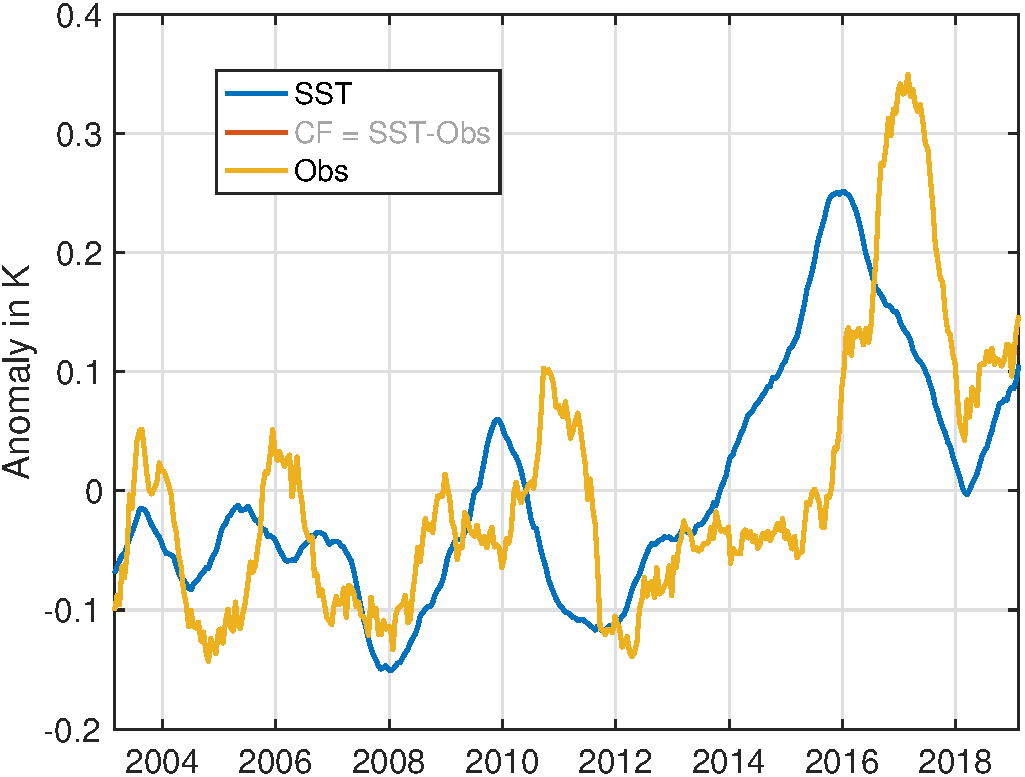
\includegraphics[width=0.7\linewidth]{./Figs/Pdf/tseries_sst_obs_global.pdf}
\end{center}
\end{frame}


\begin{frame}[label={sec:org08646cf}]{Now Add Cloud Forcing}
\begin{center}
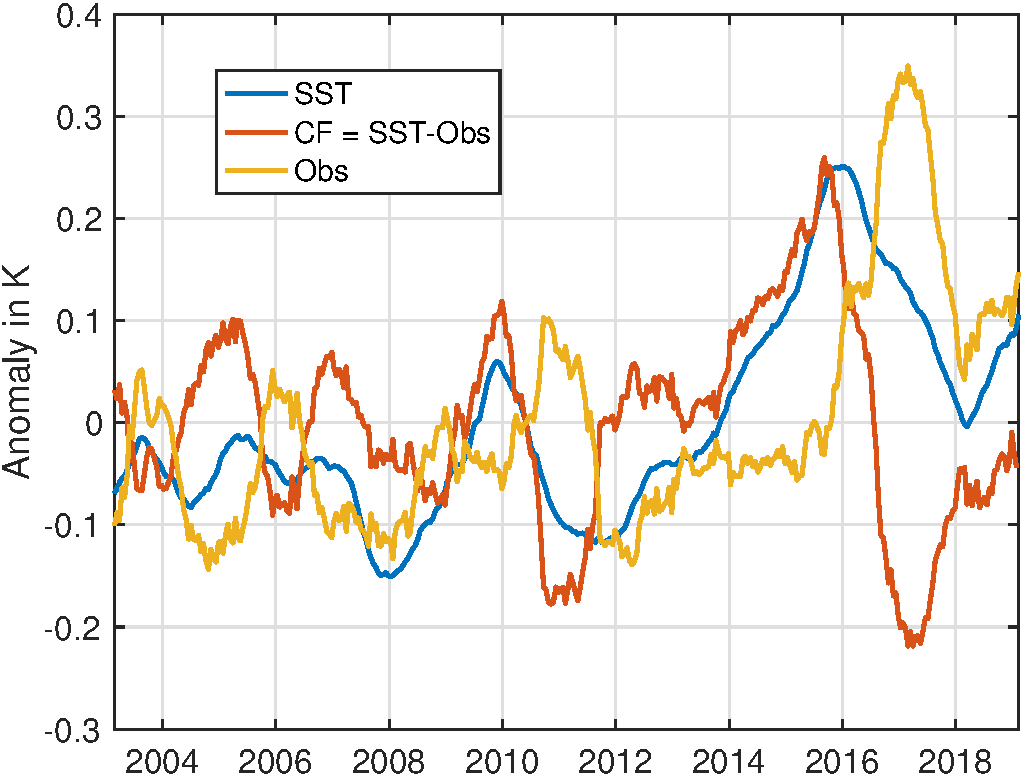
\includegraphics[width=0.7\linewidth]{./Figs/Pdf/tseries_sst_cf_obs_global.pdf}
\end{center}

\small 
\begin{itemize}
\item Note sharp CF drop at SST peak anomaly
\end{itemize}
\end{frame}

\begin{frame}[label={sec:orge4a7257}]{Delay of BTobs Anomaly to SST Anomaly}
\begin{center}
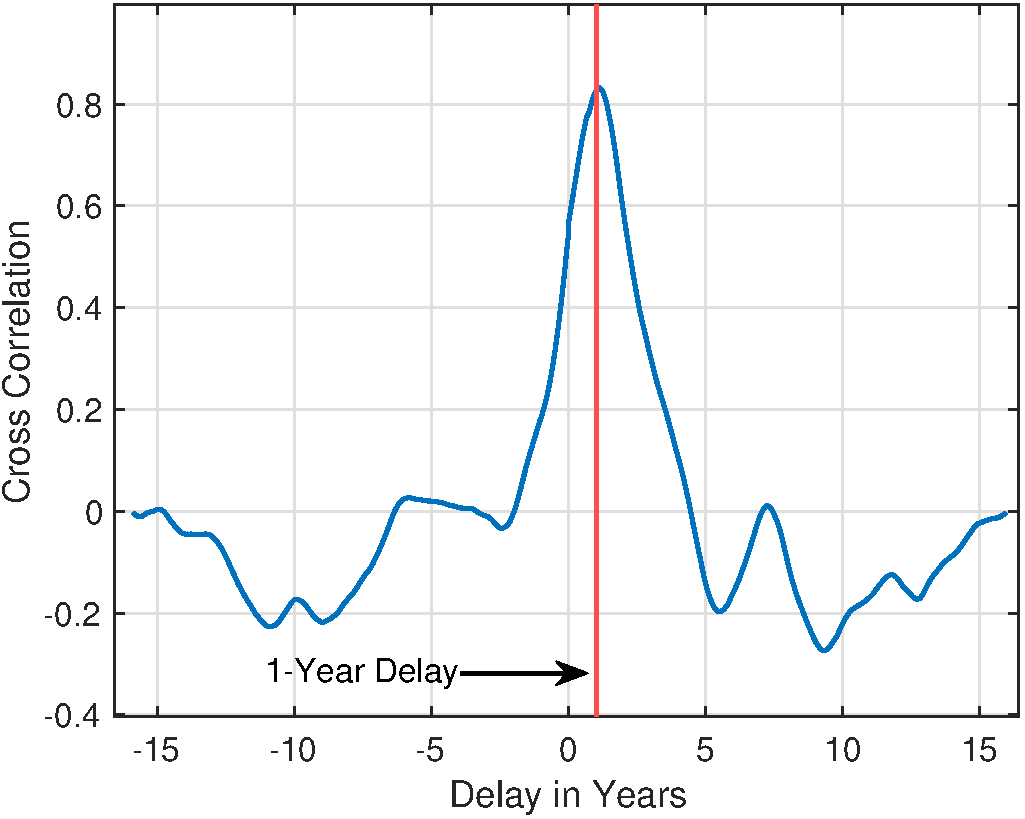
\includegraphics[width=0.7\linewidth]{./Figs/Pdf/ocean_btobs_delay_from_sst.pdf}
\end{center}

\small 
\begin{itemize}
\item Almost exactly a 1-year delay in BTobs (clear trend) from SST
\end{itemize}
\end{frame}

\begin{frame}[label={sec:org1b66617}]{Examine Time Dependence of CF vs SST Anomaly}
\vspace{-0.15in}
\begin{center}
\includegraphics[width=0.7\linewidth]{./Figs/Png/cf_vs_sst_vs_year.png}
\end{center}

\vspace{-0.15in}
\footnotesize
\begin{itemize}
\item At peak of ENSO CF drops very quickly
\item Overshoots
\item Then back to normal, BUT, of course, SST has gone up by a tremendous amount in a short time: 0.15K
\end{itemize}
\end{frame}

\begin{frame}[label={sec:orgb37755f}]{CF vs ENSO Index}
\begin{center}
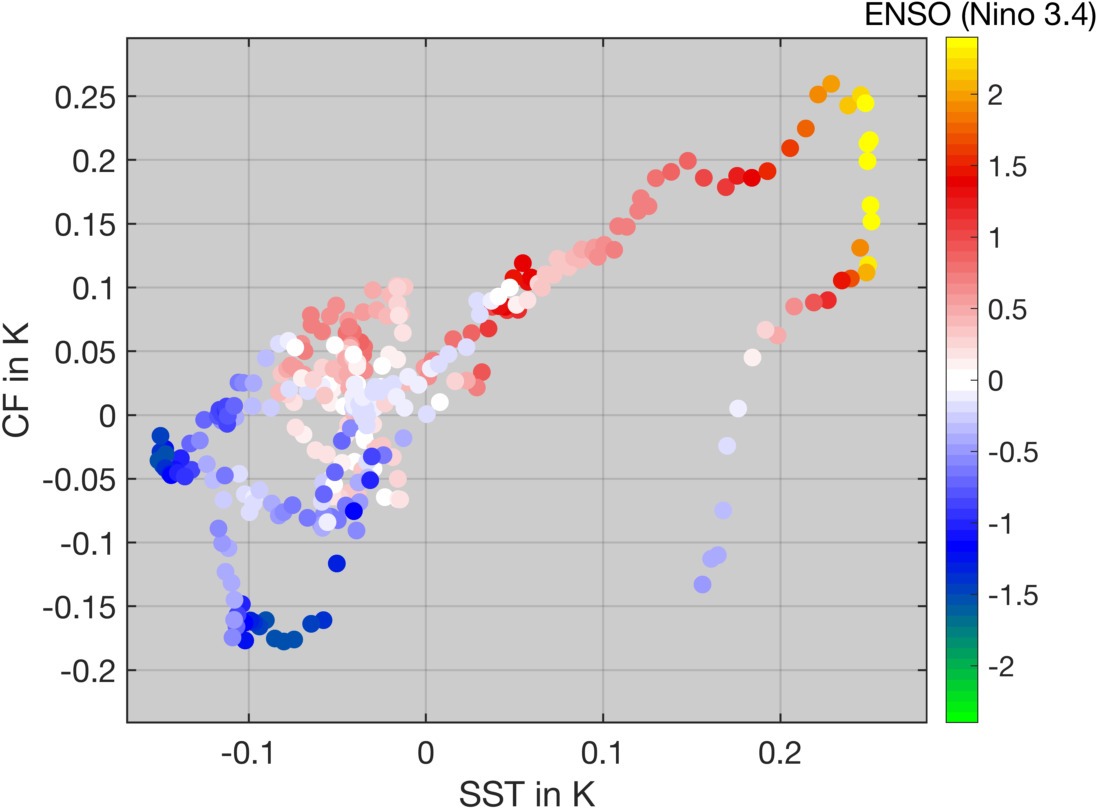
\includegraphics[width=0.7\linewidth]{./Figs/Png/cf_vs_sst_vs_enso_v2.png}
\end{center}

\footnotesize
\begin{itemize}
\item ENSO returns to normal, CF returns
\end{itemize}
\end{frame}

\begin{frame}[label={sec:orgd9a47e3}]{Climate Model Cloud Trends (Trenberth, 2009)}
\begin{center}
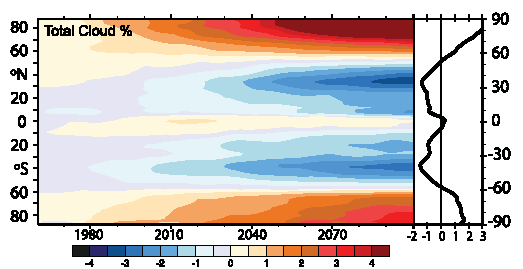
\includegraphics[width=0.9\linewidth]{./Figsc/Pdf/trenberth2009_clouds_top.pdf}
\end{center}
\end{frame}

\begin{frame}[label={sec:orgaf042e2}]{AIRS CF (Scales about right)}
\begin{columns}
\begin{column}{0.55\columnwidth}
\begin{block}{Climate Model C(fraction) Trend}
\vspace{-0.15in}
\begin{center}
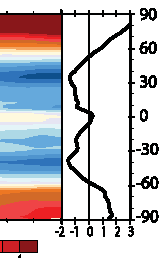
\includegraphics[width=0.7\linewidth]{./Figsc/Pdf/trenberth_total_only.pdf}
\end{center}
\end{block}
\end{column}


\begin{column}{0.55\columnwidth}
\begin{block}{AIRS CF Trend}
\begin{center}
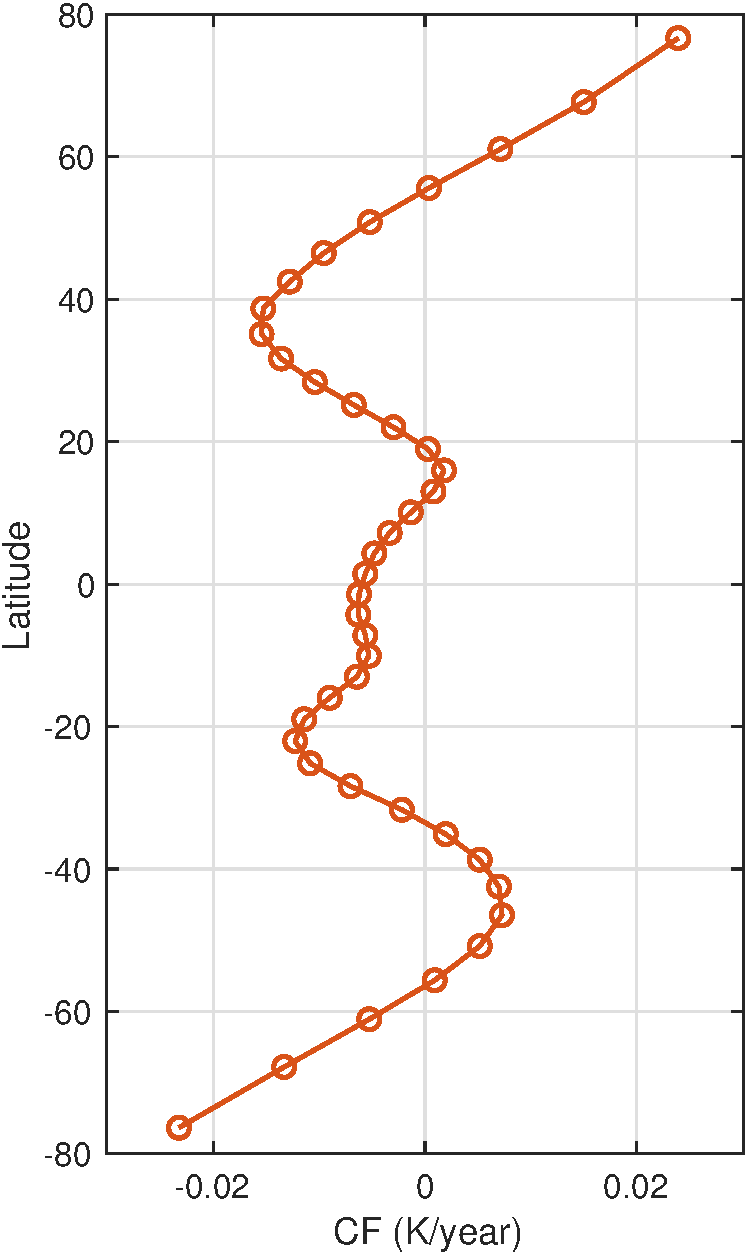
\includegraphics[width=0.6\linewidth]{./Figsc/Pdf/new_trend_rand_stats_1231_and_2161_era_clr_minus_obs_smoothed.pdf}
\end{center}
\end{block}
\end{column}
\end{columns}
\end{frame}
\end{document}